\chapter{Vectorization}
 \label{chap:vec}
 
 To mitigate the storage of duplicated data in both the \emph{PyNEST} and \emph{NestKernel} sides, we thought about decomposing the models into segments that are simple to generate from the perspective of the code generator and yet independent, which makes it more efficient in the \emph{JIT} code generation context. In computer science, we refer to this decomposition as \emph{modularity}. The idea behind it is to consider the model as an aggregation of blocks, and these blocks are assembled during the progress of the simulation script upon calling the \texttt{nest.Create}, \texttt{nest.Connect} and \texttt{nest.Simulate} functions. Each model will start with a \emph{dummy} instance of the \texttt{Node} class in the \emph{NestKernel} that only has pointers to these blocks, which they will be assigned  separately and independently during the simulation. Such blocks may extend the \emph{dummy} instance by new attributes like new \emph{Parameters} and new \emph{States}, or even new functions related to updating the state of the model, delivering emitted events and registering connections. Basically, a valid perfect partition of the model into segments is the partition that aligns with the \texttt{nest.Create}, \texttt{nest.Connect} and \texttt{nest.Simulate}. When calling the \texttt{nest.Create}, we only require the \emph{Parameter} and \emph{State} blocks to be assigned to the model. On \texttt{nest.Connect}, we extend the model by new functions that support the connectivity of the neuron with the synapse. Finally, by calling \texttt{nest.Simulate}, we append the \texttt{update} block. This partition might not be always perfect and depending on the chosen model, we may require a different segmentation and a more detailed analysis to create the blocks. 


A problem might rise with this approach is that when creating $n$ instances from the model. In the context of modularity and as depicted in the \autoref{fig:moduliarity_vectorization} in the left part, it means that each \emph{State} block must be constructed separately, and each block must be assigned to each instance of the model. So assuming the time for creating a \emph{State} block takes $c$ times and biding each instance of the model with the block takes $a$ times and $l$ is the time needed for creating each node separately. Therefore, if we have $n$ instances, then overall we will spend $n \cdot (c + a + l)$ connecting each block with its corresponding instance. 

Here where the \emph{Vectorization} comes into play. Instead of having $n$ instances of the \emph{State} block, we only use one block that is \emph{shared} among all other instances of the model. Thus, the \emph{State} block is now vectorized, which means it has a vector of attributes where each entry in the vector corresponds to an instance of the model at the position $i$. Again, if we have $n$ instances then the overall time needed for creating the instance is $n (\cdot a + l) + c + r $, where $r$ is the overhead for resizing the vector and allocating space for it. It is also possible to reduce the $n \cdot a$ part in which we just have a central entity that has direct access to the blocks and instances of the model. Therefore, the $a$ term will completely vanish, and the overall time required for the \texttt{nest.Create} to finish will be  $ \approx n \cdot l + c + r $. In \autoref{fig:central_entity}, we illustrate the best way how the modularity and vectorization may work together to achieve a simple and flexible data structure for handling models in the \emph{NestKernel}. The \emph{central entity} in this context may be the \texttt{Model} class in the \texttt{NestKernel}, and it only exists once per thread. The instances of the \texttt{Node} class are depicted in circles, and they all share the \emph{central entity} which has direct access to the \emph{State}, \emph{Parameter} blocks. Each node has a \texttt{local\_id} and with it only it can retrieve information about the current stored values of the \emph{State} and the \emph{Parameter} at the corresponding positions.
 
In this thesis, we will only focus on implementing the \emph{Vectorization} concept for the models and show that it is possible to integrate the \emph{Vectorization} design in the \emph{NestKernel} without drastically breaking its workflow.

In this chapter, we introduce a naive solution and discuss its drawbacks, and then we show a better solution that respects certain requirements coming from the \emph{NestKernel} and finally discuss the current limitations and how is it possible to mitigate them.
 
 \begin{figure}[ht!]
 \centering 
\tikzset{every picture/.style={line width=0.75pt}} %set default line width to 0.75pt        



\tikzset{every picture/.style={line width=0.75pt}} %set default line width to 0.75pt        

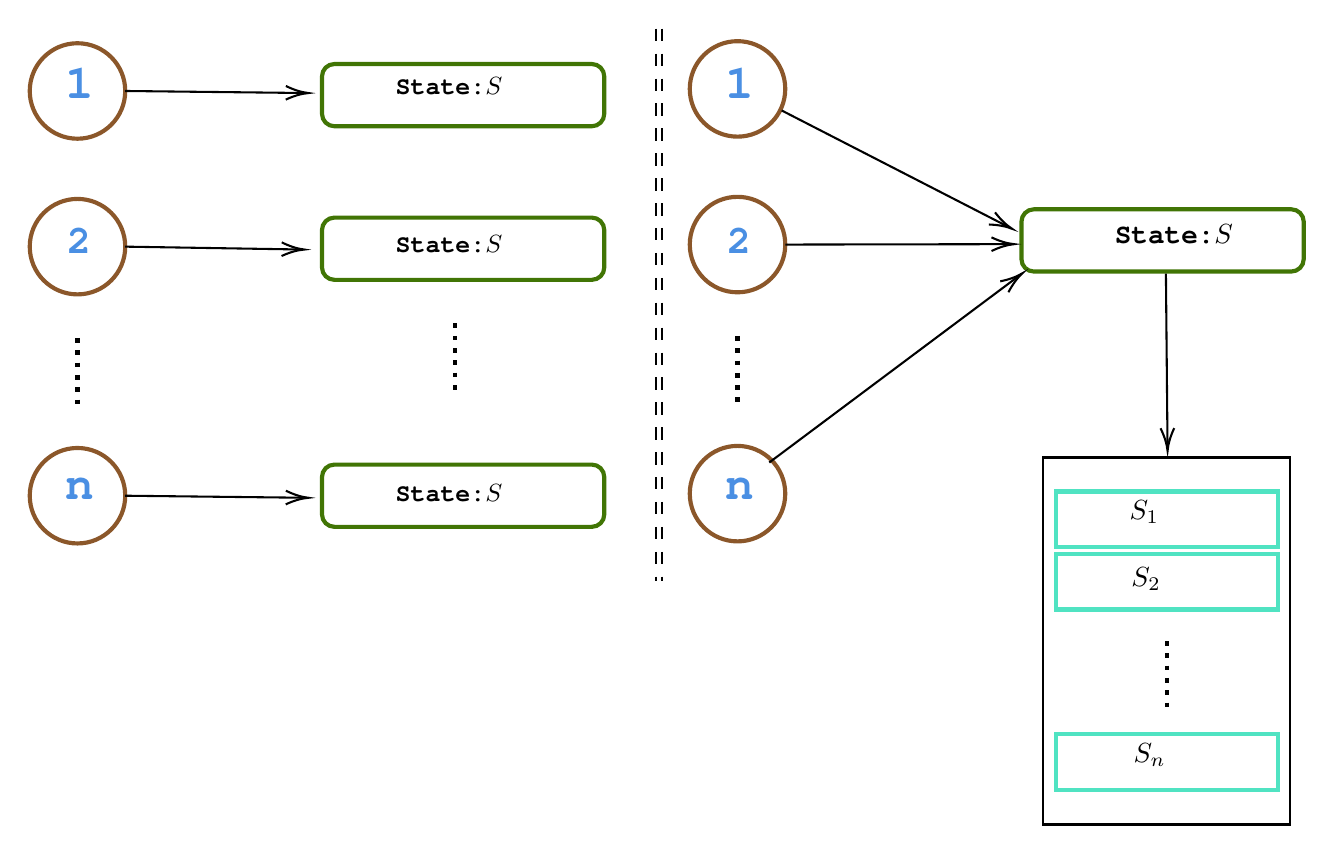
\begin{tikzpicture}[x=0.75pt,y=0.75pt,yscale=-1,xscale=1]
%uncomment if require: \path (0,407); %set diagram left start at 0, and has height of 407

%Straight Lines [id:da55454641213535] 
\draw  [dash pattern={on 4.5pt off 4.5pt}]  (320.3,5) -- (320.3,271)(317.3,5) -- (317.3,271) ;
%Shape: Circle [id:dp8702862076063935] 
\draw  [color={rgb, 255:red, 139; green, 87; blue, 42 }  ,draw opacity=1 ][line width=1.5]  (15.5,35) .. controls (15.5,22.3) and (25.8,12) .. (38.5,12) .. controls (51.2,12) and (61.5,22.3) .. (61.5,35) .. controls (61.5,47.7) and (51.2,58) .. (38.5,58) .. controls (25.8,58) and (15.5,47.7) .. (15.5,35) -- cycle ;
%Shape: Circle [id:dp7392015554996889] 
\draw  [color={rgb, 255:red, 139; green, 87; blue, 42 }  ,draw opacity=1 ][line width=1.5]  (15.5,110) .. controls (15.5,97.3) and (25.8,87) .. (38.5,87) .. controls (51.2,87) and (61.5,97.3) .. (61.5,110) .. controls (61.5,122.7) and (51.2,133) .. (38.5,133) .. controls (25.8,133) and (15.5,122.7) .. (15.5,110) -- cycle ;
%Shape: Circle [id:dp2317183663755913] 
\draw  [color={rgb, 255:red, 139; green, 87; blue, 42 }  ,draw opacity=1 ][line width=1.5]  (15.5,230) .. controls (15.5,217.3) and (25.8,207) .. (38.5,207) .. controls (51.2,207) and (61.5,217.3) .. (61.5,230) .. controls (61.5,242.7) and (51.2,253) .. (38.5,253) .. controls (25.8,253) and (15.5,242.7) .. (15.5,230) -- cycle ;
%Straight Lines [id:da38894787507587125] 
\draw [line width=1.5]  [dash pattern={on 1.69pt off 2.76pt}]  (38.5,154) -- (38.5,189) ;
%Shape: Circle [id:dp12642715215459321] 
\draw  [color={rgb, 255:red, 139; green, 87; blue, 42 }  ,draw opacity=1 ][line width=1.5]  (333.5,34) .. controls (333.5,21.3) and (343.8,11) .. (356.5,11) .. controls (369.2,11) and (379.5,21.3) .. (379.5,34) .. controls (379.5,46.7) and (369.2,57) .. (356.5,57) .. controls (343.8,57) and (333.5,46.7) .. (333.5,34) -- cycle ;
%Shape: Circle [id:dp810070044573385] 
\draw  [color={rgb, 255:red, 139; green, 87; blue, 42 }  ,draw opacity=1 ][line width=1.5]  (333.5,109) .. controls (333.5,96.3) and (343.8,86) .. (356.5,86) .. controls (369.2,86) and (379.5,96.3) .. (379.5,109) .. controls (379.5,121.7) and (369.2,132) .. (356.5,132) .. controls (343.8,132) and (333.5,121.7) .. (333.5,109) -- cycle ;
%Shape: Circle [id:dp9280679238307532] 
\draw  [color={rgb, 255:red, 139; green, 87; blue, 42 }  ,draw opacity=1 ][line width=1.5]  (333.5,229) .. controls (333.5,216.3) and (343.8,206) .. (356.5,206) .. controls (369.2,206) and (379.5,216.3) .. (379.5,229) .. controls (379.5,241.7) and (369.2,252) .. (356.5,252) .. controls (343.8,252) and (333.5,241.7) .. (333.5,229) -- cycle ;
%Straight Lines [id:da15371263291441517] 
\draw [line width=1.5]  [dash pattern={on 1.69pt off 2.76pt}]  (356.5,153) -- (356.5,188) ;
%Rounded Rect [id:dp7336088599348931] 
\draw  [color={rgb, 255:red, 65; green, 117; blue, 5 }  ,draw opacity=1 ][line width=1.5]  (156.3,28) .. controls (156.3,24.69) and (158.99,22) .. (162.3,22) -- (286.3,22) .. controls (289.61,22) and (292.3,24.69) .. (292.3,28) -- (292.3,46) .. controls (292.3,49.31) and (289.61,52) .. (286.3,52) -- (162.3,52) .. controls (158.99,52) and (156.3,49.31) .. (156.3,46) -- cycle ;
%Rounded Rect [id:dp7973935185576317] 
\draw  [color={rgb, 255:red, 65; green, 117; blue, 5 }  ,draw opacity=1 ][line width=1.5]  (156.3,102) .. controls (156.3,98.69) and (158.99,96) .. (162.3,96) -- (286.3,96) .. controls (289.61,96) and (292.3,98.69) .. (292.3,102) -- (292.3,120) .. controls (292.3,123.31) and (289.61,126) .. (286.3,126) -- (162.3,126) .. controls (158.99,126) and (156.3,123.31) .. (156.3,120) -- cycle ;
%Rounded Rect [id:dp24096719551443324] 
\draw  [color={rgb, 255:red, 65; green, 117; blue, 5 }  ,draw opacity=1 ][line width=1.5]  (156.3,221) .. controls (156.3,217.69) and (158.99,215) .. (162.3,215) -- (286.3,215) .. controls (289.61,215) and (292.3,217.69) .. (292.3,221) -- (292.3,239) .. controls (292.3,242.31) and (289.61,245) .. (286.3,245) -- (162.3,245) .. controls (158.99,245) and (156.3,242.31) .. (156.3,239) -- cycle ;
%Straight Lines [id:da10099325819440153] 
\draw [line width=1.5]  [dash pattern={on 1.69pt off 2.76pt}]  (220.3,147) -- (220.3,182) ;
%Straight Lines [id:da41136869587104075] 
\draw    (61.5,35) -- (147.8,35.98) ;
\draw [shift={(149.8,36)}, rotate = 180.65] [color={rgb, 255:red, 0; green, 0; blue, 0 }  ][line width=0.75]    (10.93,-3.29) .. controls (6.95,-1.4) and (3.31,-0.3) .. (0,0) .. controls (3.31,0.3) and (6.95,1.4) .. (10.93,3.29)   ;
%Straight Lines [id:da2870462219518801] 
\draw    (61.5,110) -- (145.8,111.37) ;
\draw [shift={(147.8,111.4)}, rotate = 180.93] [color={rgb, 255:red, 0; green, 0; blue, 0 }  ][line width=0.75]    (10.93,-3.29) .. controls (6.95,-1.4) and (3.31,-0.3) .. (0,0) .. controls (3.31,0.3) and (6.95,1.4) .. (10.93,3.29)   ;
%Straight Lines [id:da05926760400293096] 
\draw    (61.5,230) -- (147.8,230.98) ;
\draw [shift={(149.8,231)}, rotate = 180.65] [color={rgb, 255:red, 0; green, 0; blue, 0 }  ][line width=0.75]    (10.93,-3.29) .. controls (6.95,-1.4) and (3.31,-0.3) .. (0,0) .. controls (3.31,0.3) and (6.95,1.4) .. (10.93,3.29)   ;
%Rounded Rect [id:dp5327938345694794] 
\draw  [color={rgb, 255:red, 65; green, 117; blue, 5 }  ,draw opacity=1 ][line width=1.5]  (493.3,98) .. controls (493.3,94.69) and (495.99,92) .. (499.3,92) -- (623.3,92) .. controls (626.61,92) and (629.3,94.69) .. (629.3,98) -- (629.3,116) .. controls (629.3,119.31) and (626.61,122) .. (623.3,122) -- (499.3,122) .. controls (495.99,122) and (493.3,119.31) .. (493.3,116) -- cycle ;
%Straight Lines [id:da24962287312365405] 
\draw    (377.8,44.4) -- (487.02,100.49) ;
\draw [shift={(488.8,101.4)}, rotate = 207.18] [color={rgb, 255:red, 0; green, 0; blue, 0 }  ][line width=0.75]    (10.93,-3.29) .. controls (6.95,-1.4) and (3.31,-0.3) .. (0,0) .. controls (3.31,0.3) and (6.95,1.4) .. (10.93,3.29)   ;
%Straight Lines [id:da0756642394053797] 
\draw    (379.5,109) -- (487.8,108.8) ;
\draw [shift={(489.8,108.8)}, rotate = 179.9] [color={rgb, 255:red, 0; green, 0; blue, 0 }  ][line width=0.75]    (10.93,-3.29) .. controls (6.95,-1.4) and (3.31,-0.3) .. (0,0) .. controls (3.31,0.3) and (6.95,1.4) .. (10.93,3.29)   ;
%Straight Lines [id:da5803854131041157] 
\draw    (371.8,214) -- (492.2,124) ;
\draw [shift={(493.8,122.8)}, rotate = 143.22] [color={rgb, 255:red, 0; green, 0; blue, 0 }  ][line width=0.75]    (10.93,-3.29) .. controls (6.95,-1.4) and (3.31,-0.3) .. (0,0) .. controls (3.31,0.3) and (6.95,1.4) .. (10.93,3.29)   ;
%Shape: Rectangle [id:dp8303325304778635] 
\draw  [color={rgb, 255:red, 80; green, 227; blue, 194 }  ,draw opacity=1 ][line width=1.5]  (509.9,228) -- (616.7,228) -- (616.7,254.8) -- (509.9,254.8) -- cycle ;
%Straight Lines [id:da8940404822400119] 
\draw [line width=1.5]  [dash pattern={on 1.69pt off 2.76pt}]  (563.3,300) -- (563.3,335) ;
%Shape: Rectangle [id:dp9884603058041568] 
\draw  [color={rgb, 255:red, 80; green, 227; blue, 194 }  ,draw opacity=1 ][line width=1.5]  (509.9,258) -- (616.7,258) -- (616.7,284.8) -- (509.9,284.8) -- cycle ;
%Shape: Rectangle [id:dp5121717716613057] 
\draw  [color={rgb, 255:red, 80; green, 227; blue, 194 }  ,draw opacity=1 ][line width=1.5]  (509.9,345) -- (616.7,345) -- (616.7,371.8) -- (509.9,371.8) -- cycle ;
%Shape: Rectangle [id:dp907132490388713] 
\draw   (503.8,211.6) -- (622.8,211.6) -- (622.8,388.4) -- (503.8,388.4) -- cycle ;
%Straight Lines [id:da8778275970204104] 
\draw    (562.9,123) -- (563.68,206.4) ;
\draw [shift={(563.7,208.4)}, rotate = 269.46] [color={rgb, 255:red, 0; green, 0; blue, 0 }  ][line width=0.75]    (10.93,-3.29) .. controls (6.95,-1.4) and (3.31,-0.3) .. (0,0) .. controls (3.31,0.3) and (6.95,1.4) .. (10.93,3.29)   ;

% Text Node
\draw (31,23) node [anchor=north west][inner sep=0.75pt]   [align=left] {{\fontfamily{pcr}\selectfont {\LARGE \textcolor[rgb]{0.29,0.56,0.89}{\textbf{1}}}}};
% Text Node
\draw (32,100) node [anchor=north west][inner sep=0.75pt]   [align=left] {{\fontfamily{pcr}\selectfont {\Large \textcolor[rgb]{0.29,0.56,0.89}{\textbf{2}}}}};
% Text Node
\draw (31,220) node [anchor=north west][inner sep=0.75pt]   [align=left] {{\fontfamily{pcr}\selectfont {\LARGE \textcolor[rgb]{0.29,0.56,0.89}{\textbf{n}}}}};
% Text Node
\draw (349,23) node [anchor=north west][inner sep=0.75pt]   [align=left] {{\fontfamily{pcr}\selectfont {\LARGE \textcolor[rgb]{0.29,0.56,0.89}{\textbf{1}}}}};
% Text Node
\draw (350,100) node [anchor=north west][inner sep=0.75pt]   [align=left] {{\fontfamily{pcr}\selectfont {\Large \textcolor[rgb]{0.29,0.56,0.89}{\textbf{2}}}}};
% Text Node
\draw (349,220) node [anchor=north west][inner sep=0.75pt]   [align=left] {{\fontfamily{pcr}\selectfont {\LARGE \textcolor[rgb]{0.29,0.56,0.89}{\textbf{n}}}}};
% Text Node
\draw (536.8,98) node [anchor=north west][inner sep=0.75pt]   [align=left] {{\fontfamily{pcr}\selectfont \textbf{State:$S$}}};
% Text Node
\draw (190.3,27) node [anchor=north west][inner sep=0.75pt]   [align=left] {{\small {\fontfamily{pcr}\selectfont \textbf{State:$S$}}}};
% Text Node
\draw (190.3,103) node [anchor=north west][inner sep=0.75pt]   [align=left] {{\small {\fontfamily{pcr}\selectfont \textbf{State:$S$ }}}};
% Text Node
\draw (190.3,223) node [anchor=north west][inner sep=0.75pt]   [align=left] {{\small {\fontfamily{pcr}\selectfont \textbf{State:$S$ }}}};
% Text Node
\draw (544.8,263) node [anchor=north west][inner sep=0.75pt]   [align=left] {$S_2$};
% Text Node
\draw (543.9,231) node [anchor=north west][inner sep=0.75pt]   [align=left] {$S_{1}$};
% Text Node
\draw (545.9,348) node [anchor=north west][inner sep=0.75pt]   [align=left] {$S_{n}$};


\end{tikzpicture}

\caption{Modularity and Vectorization: The left part represents the current implementation of the models in the \emph{NestKenel}. We have $n$ instances of the model and each has its own \emph{state} block with an attribute $S$. In the right, we have the suggested idea using \emph{vectorization}. All instances share the same \emph{state} block, and instead of having $n$ separated attributes, the attributes are aggregated in a single array with size $n$.}
\label{fig:moduliarity_vectorization}
\end{figure}


\begin{figure}[ht!]
    \centering
    

\tikzset{every picture/.style={line width=0.75pt}} %set default line width to 0.75pt        

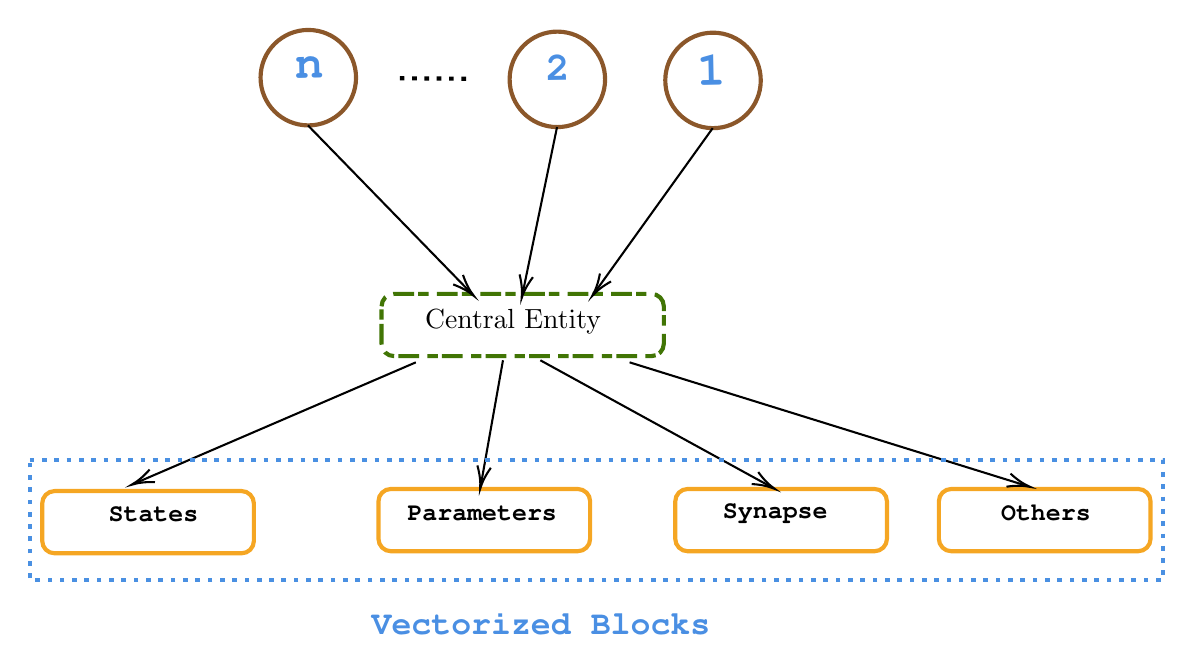
\begin{tikzpicture}[x=0.75pt,y=0.75pt,yscale=-1,xscale=1]
%uncomment if require: \path (0,498); %set diagram left start at 0, and has height of 498

%Shape: Circle [id:dp8800281867294899] 
\draw  [color={rgb, 255:red, 139; green, 87; blue, 42 }  ,draw opacity=1 ][line width=1.5]  (422.15,8.16) .. controls (434.86,8.25) and (445.08,18.62) .. (445,31.32) .. controls (444.91,44.02) and (434.54,54.25) .. (421.84,54.16) .. controls (409.14,54.08) and (398.91,43.71) .. (399,31.01) .. controls (399.08,18.3) and (409.45,8.08) .. (422.15,8.16) -- cycle ;
%Shape: Circle [id:dp5741608202490043] 
\draw  [color={rgb, 255:red, 139; green, 87; blue, 42 }  ,draw opacity=1 ][line width=1.5]  (347.16,7.65) .. controls (359.86,7.74) and (370.09,18.11) .. (370,30.81) .. controls (369.91,43.51) and (359.55,53.74) .. (346.84,53.65) .. controls (334.14,53.57) and (323.91,43.2) .. (324,30.5) .. controls (324.09,17.79) and (334.45,7.57) .. (347.16,7.65) -- cycle ;
%Shape: Circle [id:dp5967106723538562] 
\draw  [color={rgb, 255:red, 139; green, 87; blue, 42 }  ,draw opacity=1 ][line width=1.5]  (227.16,6.84) .. controls (239.86,6.92) and (250.09,17.29) .. (250,29.99) .. controls (249.92,42.7) and (239.55,52.92) .. (226.85,52.84) .. controls (214.14,52.75) and (203.92,42.38) .. (204,29.68) .. controls (204.09,16.98) and (214.46,6.75) .. (227.16,6.84) -- cycle ;
%Straight Lines [id:da29612448901916677] 
\draw [line width=1.5]  [dash pattern={on 1.69pt off 2.76pt}]  (303,30.35) -- (268,30.12) ;
%Rounded Rect [id:dp817325473851275] 
\draw  [color={rgb, 255:red, 65; green, 117; blue, 5 }  ,draw opacity=1 ][dash pattern={on 3.75pt off 3pt on 7.5pt off 1.5pt}][line width=1.5]  (262.3,140) .. controls (262.3,136.69) and (264.99,134) .. (268.3,134) -- (392.3,134) .. controls (395.61,134) and (398.3,136.69) .. (398.3,140) -- (398.3,158) .. controls (398.3,161.31) and (395.61,164) .. (392.3,164) -- (268.3,164) .. controls (264.99,164) and (262.3,161.31) .. (262.3,158) -- cycle ;
%Straight Lines [id:da2876052096679098] 
\draw    (226.85,52.84) -- (305.41,133.57) ;
\draw [shift={(306.8,135)}, rotate = 225.78] [color={rgb, 255:red, 0; green, 0; blue, 0 }  ][line width=0.75]    (10.93,-3.29) .. controls (6.95,-1.4) and (3.31,-0.3) .. (0,0) .. controls (3.31,0.3) and (6.95,1.4) .. (10.93,3.29)   ;
%Straight Lines [id:da21493226208984018] 
\draw    (346.84,53.65) -- (330.21,134.04) ;
\draw [shift={(329.8,136)}, rotate = 281.69] [color={rgb, 255:red, 0; green, 0; blue, 0 }  ][line width=0.75]    (10.93,-3.29) .. controls (6.95,-1.4) and (3.31,-0.3) .. (0,0) .. controls (3.31,0.3) and (6.95,1.4) .. (10.93,3.29)   ;
%Straight Lines [id:da8022220076746627] 
\draw    (421.84,54.16) -- (364.97,133.38) ;
\draw [shift={(363.8,135)}, rotate = 305.68] [color={rgb, 255:red, 0; green, 0; blue, 0 }  ][line width=0.75]    (10.93,-3.29) .. controls (6.95,-1.4) and (3.31,-0.3) .. (0,0) .. controls (3.31,0.3) and (6.95,1.4) .. (10.93,3.29)   ;
%Rounded Rect [id:dp8286030826901589] 
\draw  [color={rgb, 255:red, 245; green, 166; blue, 35 }  ,draw opacity=1 ][line width=1.5]  (98.8,235) .. controls (98.8,231.69) and (101.49,229) .. (104.8,229) -- (194.8,229) .. controls (198.11,229) and (200.8,231.69) .. (200.8,235) -- (200.8,253) .. controls (200.8,256.31) and (198.11,259) .. (194.8,259) -- (104.8,259) .. controls (101.49,259) and (98.8,256.31) .. (98.8,253) -- cycle ;
%Rounded Rect [id:dp8880914545431386] 
\draw  [color={rgb, 255:red, 245; green, 166; blue, 35 }  ,draw opacity=1 ][line width=1.5]  (260.8,234) .. controls (260.8,230.69) and (263.49,228) .. (266.8,228) -- (356.8,228) .. controls (360.11,228) and (362.8,230.69) .. (362.8,234) -- (362.8,252) .. controls (362.8,255.31) and (360.11,258) .. (356.8,258) -- (266.8,258) .. controls (263.49,258) and (260.8,255.31) .. (260.8,252) -- cycle ;
%Rounded Rect [id:dp6892742079278225] 
\draw  [color={rgb, 255:red, 245; green, 166; blue, 35 }  ,draw opacity=1 ][line width=1.5]  (403.8,234) .. controls (403.8,230.69) and (406.49,228) .. (409.8,228) -- (499.8,228) .. controls (503.11,228) and (505.8,230.69) .. (505.8,234) -- (505.8,252) .. controls (505.8,255.31) and (503.11,258) .. (499.8,258) -- (409.8,258) .. controls (406.49,258) and (403.8,255.31) .. (403.8,252) -- cycle ;
%Rounded Rect [id:dp7219152508117417] 
\draw  [color={rgb, 255:red, 245; green, 166; blue, 35 }  ,draw opacity=1 ][line width=1.5]  (530.8,234) .. controls (530.8,230.69) and (533.49,228) .. (536.8,228) -- (626.8,228) .. controls (630.11,228) and (632.8,230.69) .. (632.8,234) -- (632.8,252) .. controls (632.8,255.31) and (630.11,258) .. (626.8,258) -- (536.8,258) .. controls (533.49,258) and (530.8,255.31) .. (530.8,252) -- cycle ;
%Straight Lines [id:da25677235530600573] 
\draw    (278.8,167) -- (143.64,225.21) ;
\draw [shift={(141.8,226)}, rotate = 336.7] [color={rgb, 255:red, 0; green, 0; blue, 0 }  ][line width=0.75]    (10.93,-3.29) .. controls (6.95,-1.4) and (3.31,-0.3) .. (0,0) .. controls (3.31,0.3) and (6.95,1.4) .. (10.93,3.29)   ;
%Straight Lines [id:da5461915180486876] 
\draw    (320.8,166) -- (310.15,226.03) ;
\draw [shift={(309.8,228)}, rotate = 280.06] [color={rgb, 255:red, 0; green, 0; blue, 0 }  ][line width=0.75]    (10.93,-3.29) .. controls (6.95,-1.4) and (3.31,-0.3) .. (0,0) .. controls (3.31,0.3) and (6.95,1.4) .. (10.93,3.29)   ;
%Straight Lines [id:da447748925987298] 
\draw    (338.8,166) -- (450.05,227.04) ;
\draw [shift={(451.8,228)}, rotate = 208.75] [color={rgb, 255:red, 0; green, 0; blue, 0 }  ][line width=0.75]    (10.93,-3.29) .. controls (6.95,-1.4) and (3.31,-0.3) .. (0,0) .. controls (3.31,0.3) and (6.95,1.4) .. (10.93,3.29)   ;
%Straight Lines [id:da09082598278343812] 
\draw    (381.8,167) -- (572.89,226.41) ;
\draw [shift={(574.8,227)}, rotate = 197.27] [color={rgb, 255:red, 0; green, 0; blue, 0 }  ][line width=0.75]    (10.93,-3.29) .. controls (6.95,-1.4) and (3.31,-0.3) .. (0,0) .. controls (3.31,0.3) and (6.95,1.4) .. (10.93,3.29)   ;
%Shape: Rectangle [id:dp8214226950203147] 
\draw  [color={rgb, 255:red, 74; green, 144; blue, 226 }  ,draw opacity=1 ][dash pattern={on 1.69pt off 2.76pt}][line width=1.5]  (92.8,214) -- (638.8,214) -- (638.8,272) -- (92.8,272) -- cycle ;

% Text Node
\draw (412.67,18.30) node [anchor=north west][inner sep=0.75pt]  [rotate=-358.84] [align=left] {{\fontfamily{pcr}\selectfont {\LARGE \textcolor[rgb]{0.29,0.56,0.89}{\textbf{1}}}}};
% Text Node
\draw (339.79,18.27) node [anchor=north west][inner sep=0.75pt]  [rotate=-359.07] [align=left] {{\fontfamily{pcr}\selectfont {\Large \textcolor[rgb]{0.29,0.56,0.89}{\textbf{2}}}}};
% Text Node
\draw (219.13,18.30) node [anchor=north west][inner sep=0.75pt]  [rotate=-358.67] [align=left] {{\fontfamily{pcr}\selectfont {\LARGE \textcolor[rgb]{0.29,0.56,0.89}{\textbf{n}}}}};
% Text Node
\draw (281.8,140) node [anchor=north west][inner sep=0.75pt]   [align=left] {Central Entity};
% Text Node
\draw (129.3,235) node [anchor=north west][inner sep=0.75pt]   [align=left] {{\fontfamily{pcr}\selectfont \textbf{{\small States}}}};
% Text Node
\draw (273.3,235) node [anchor=north west][inner sep=0.75pt]   [align=left] {{\fontfamily{pcr}\selectfont {\small \textbf{Parameters}}}};
% Text Node
\draw (425.3,234) node [anchor=north west][inner sep=0.75pt]   [align=left] {{\small \textbf{{\fontfamily{pcr}\selectfont Synapse}}}};
% Text Node
\draw (559.3,234) node [anchor=north west][inner sep=0.75pt]   [align=left] {{\fontfamily{pcr}\selectfont {\small \textbf{Others}}}};
% Text Node
\draw (256,286) node [anchor=north west][inner sep=0.75pt]   [align=left] {{\fontfamily{pcr}\selectfont {\large \textbf{\textcolor[rgb]{0.29,0.56,0.89}{Vectorized Blocks}}}}};


\end{tikzpicture}

    \caption{Modularity with a central entity: The model is segmented into different blocks that are assembled together during the simulating. The nodes share the \emph{central entity} that manages the state of the blocks. Each of the blocks support vectorization and each of the attributes has a vector form with the size equal to the created population in the network from the specified model.}
    \label{fig:central_entity}
\end{figure}

\section{The Data Structure}

\emph{Vectorization} in a plain language is the process of rewriting an instruction that is repeating $n$ times over single entities to an instruction that is processing $k$ entities simultaneously. Usually, the term \emph{vectorization} overlaps with the \emph{SIMD} term. The \emph{SIMD} is short for \emph{single instruction/multiple data}, and it refers to the capability of the hardware components to perform the same operation on multiple data concurrently. The \autoref{fig:simd} illustrates a simple example of a \emph{SIMD} executing  four operations in parallel. Another term strongly related to high performance computing and optimization is the term \emph{speedup}. The term \emph{speedup} in the context of \emph{vectorization} is the ratio of time required by the \emph{non-vectorized} operation $T(1)$ to the time required by the \emph{vectorized} operation, executing $k$ operations at the same time noted as $T(k)$. The formula of the \emph{speedup} is the defined as $$S(k) = \frac{T(1)}{T(k)}$$. Assuming that a single instance of the operation takes $t$ units to complete and also neglect the overhead of memory access, then applying the operation on $n$ elements we have $T(1) = n \cdot t$ and $T(k) = \frac{n}{k} \cdot t$, which should imply that $$S(k) = \frac{T(1)}{T(k)} = \frac{n \cdot t}{\frac{n}{k} \cdot t} = k.$$

A \emph{speedup} of $k$ means that we load $k$ elements in the register of the processor and execute the operation $k$ times in parallel. In reality, the larger $k$ gets, the less speedup we can reach, as it strongly depends on the bandwidth of transferring the data from the main memory to the register and depending on the \emph{CPU} design and architecture, we may end up in a memory bandwidth issues, and therefore we have to be careful in which extent we should use  \emph{Vectorization}.\\




\begin{figure}[ht!]
\centering
\tikzset{every picture/.style={line width=0.75pt}} %set default line width to 0.75pt        

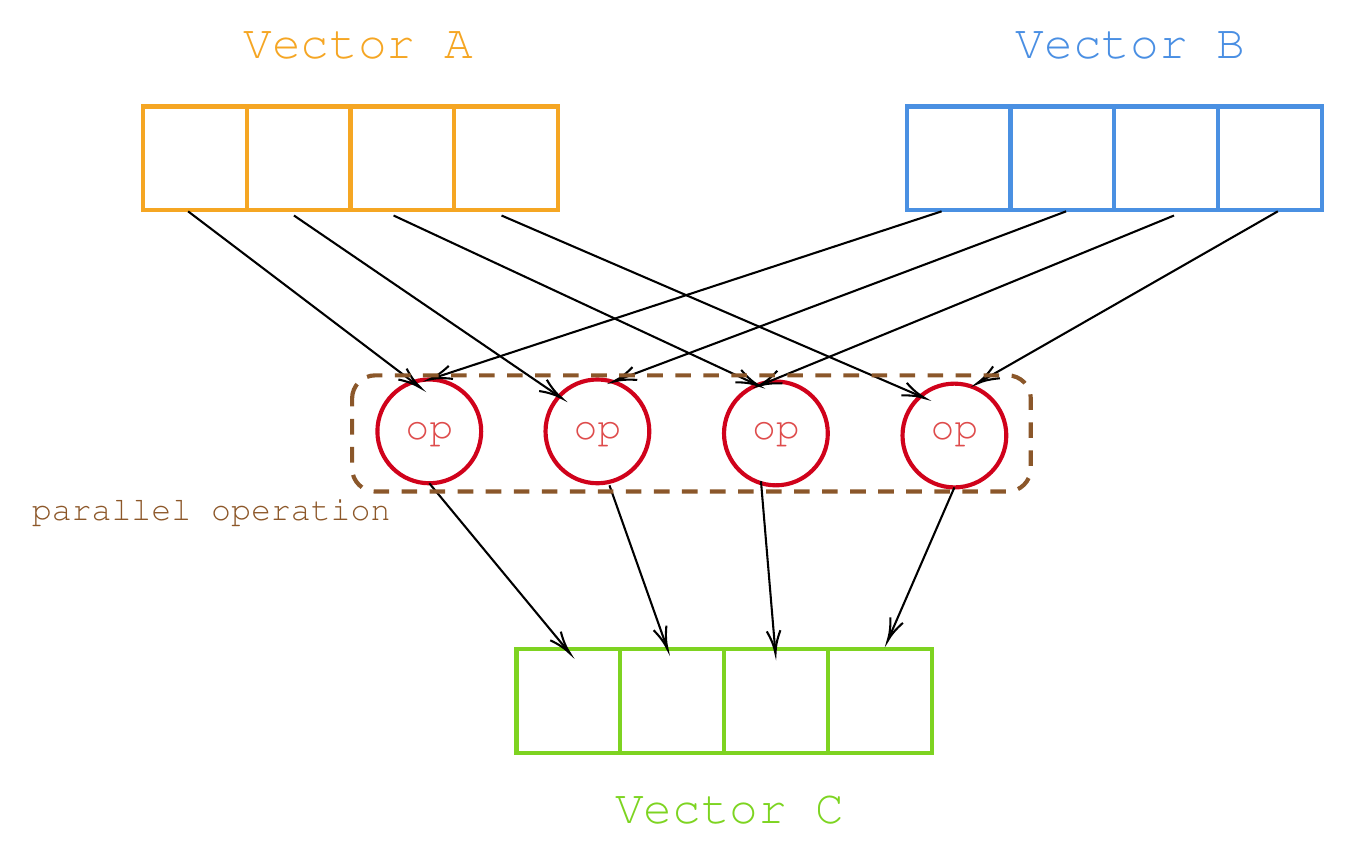
\begin{tikzpicture}[x=0.75pt,y=0.75pt,yscale=-1,xscale=1]
%uncomment if require: \path (0,489); %set diagram left start at 0, and has height of 489

%Shape: Square [id:dp46324192936376996] 
\draw  [color={rgb, 255:red, 245; green, 166; blue, 35 }  ,draw opacity=1 ][line width=1.5]  (215,42.5) -- (265,42.5) -- (265,92.5) -- (215,92.5) -- cycle ;
%Shape: Square [id:dp13405731496869033] 
\draw  [color={rgb, 255:red, 245; green, 166; blue, 35 }  ,draw opacity=1 ][line width=1.5]  (165,42.5) -- (215,42.5) -- (215,92.5) -- (165,92.5) -- cycle ;
%Shape: Square [id:dp661115292627177] 
\draw  [color={rgb, 255:red, 245; green, 166; blue, 35 }  ,draw opacity=1 ][line width=1.5]  (115,42.5) -- (165,42.5) -- (165,92.5) -- (115,92.5) -- cycle ;
%Shape: Square [id:dp745221312417149] 
\draw  [color={rgb, 255:red, 245; green, 166; blue, 35 }  ,draw opacity=1 ][line width=1.5]  (65,42.5) -- (115,42.5) -- (115,92.5) -- (65,92.5) -- cycle ;
%Shape: Square [id:dp4238228889509019] 
\draw  [color={rgb, 255:red, 74; green, 144; blue, 226 }  ,draw opacity=1 ][line width=1.5]  (583,42.5) -- (633,42.5) -- (633,92.5) -- (583,92.5) -- cycle ;
%Shape: Square [id:dp379666298904783] 
\draw  [color={rgb, 255:red, 74; green, 144; blue, 226 }  ,draw opacity=1 ][line width=1.5]  (533,42.5) -- (583,42.5) -- (583,92.5) -- (533,92.5) -- cycle ;
%Shape: Square [id:dp17007558171281212] 
\draw  [color={rgb, 255:red, 74; green, 144; blue, 226 }  ,draw opacity=1 ][line width=1.5]  (483,42.5) -- (533,42.5) -- (533,92.5) -- (483,92.5) -- cycle ;
%Shape: Square [id:dp5616212163793872] 
\draw  [color={rgb, 255:red, 74; green, 144; blue, 226 }  ,draw opacity=1 ][line width=1.5]  (433,42.5) -- (483,42.5) -- (483,92.5) -- (433,92.5) -- cycle ;
%Shape: Square [id:dp7187618339838493] 
\draw  [color={rgb, 255:red, 126; green, 211; blue, 33 }  ,draw opacity=1 ][line width=1.5]  (395,304) -- (445,304) -- (445,354) -- (395,354) -- cycle ;
%Shape: Circle [id:dp07536177233598251] 
\draw  [color={rgb, 255:red, 208; green, 2; blue, 27 }  ,draw opacity=1 ][line width=1.5]  (431,201) .. controls (431,187.19) and (442.19,176) .. (456,176) .. controls (469.81,176) and (481,187.19) .. (481,201) .. controls (481,214.81) and (469.81,226) .. (456,226) .. controls (442.19,226) and (431,214.81) .. (431,201) -- cycle ;
%Shape: Circle [id:dp30362267619189565] 
\draw  [color={rgb, 255:red, 208; green, 2; blue, 27 }  ,draw opacity=1 ][line width=1.5]  (345,200) .. controls (345,186.19) and (356.19,175) .. (370,175) .. controls (383.81,175) and (395,186.19) .. (395,200) .. controls (395,213.81) and (383.81,225) .. (370,225) .. controls (356.19,225) and (345,213.81) .. (345,200) -- cycle ;
%Shape: Circle [id:dp5510406133476184] 
\draw  [color={rgb, 255:red, 208; green, 2; blue, 27 }  ,draw opacity=1 ][line width=1.5]  (259,199) .. controls (259,185.19) and (270.19,174) .. (284,174) .. controls (297.81,174) and (309,185.19) .. (309,199) .. controls (309,212.81) and (297.81,224) .. (284,224) .. controls (270.19,224) and (259,212.81) .. (259,199) -- cycle ;
%Shape: Circle [id:dp5759692219381265] 
\draw  [color={rgb, 255:red, 208; green, 2; blue, 27 }  ,draw opacity=1 ][line width=1.5]  (178,199) .. controls (178,185.19) and (189.19,174) .. (203,174) .. controls (216.81,174) and (228,185.19) .. (228,199) .. controls (228,212.81) and (216.81,224) .. (203,224) .. controls (189.19,224) and (178,212.81) .. (178,199) -- cycle ;
%Shape: Square [id:dp45528344866305415] 
\draw  [color={rgb, 255:red, 126; green, 211; blue, 33 }  ,draw opacity=1 ][line width=1.5]  (345,304) -- (395,304) -- (395,354) -- (345,354) -- cycle ;
%Shape: Square [id:dp7610477176063681] 
\draw  [color={rgb, 255:red, 126; green, 211; blue, 33 }  ,draw opacity=1 ][line width=1.5]  (295,304) -- (345,304) -- (345,354) -- (295,354) -- cycle ;
%Shape: Square [id:dp7054962057870686] 
\draw  [color={rgb, 255:red, 126; green, 211; blue, 33 }  ,draw opacity=1 ][line width=1.5]  (245,304) -- (295,304) -- (295,354) -- (245,354) -- cycle ;
%Straight Lines [id:da9169258246854404] 
\draw    (86.8,93) -- (197.21,176.79) ;
\draw [shift={(198.8,178)}, rotate = 217.2] [color={rgb, 255:red, 0; green, 0; blue, 0 }  ][line width=0.75]    (10.93,-3.29) .. controls (6.95,-1.4) and (3.31,-0.3) .. (0,0) .. controls (3.31,0.3) and (6.95,1.4) .. (10.93,3.29)   ;
%Straight Lines [id:da31261363225043004] 
\draw    (137.8,95) -- (265.15,181.87) ;
\draw [shift={(266.8,183)}, rotate = 214.3] [color={rgb, 255:red, 0; green, 0; blue, 0 }  ][line width=0.75]    (10.93,-3.29) .. controls (6.95,-1.4) and (3.31,-0.3) .. (0,0) .. controls (3.31,0.3) and (6.95,1.4) .. (10.93,3.29)   ;
%Straight Lines [id:da26051228228325707] 
\draw    (185.8,95) -- (359.99,176.16) ;
\draw [shift={(361.8,177)}, rotate = 204.98] [color={rgb, 255:red, 0; green, 0; blue, 0 }  ][line width=0.75]    (10.93,-3.29) .. controls (6.95,-1.4) and (3.31,-0.3) .. (0,0) .. controls (3.31,0.3) and (6.95,1.4) .. (10.93,3.29)   ;
%Straight Lines [id:da19220482069259948] 
\draw    (237.8,95) -- (439.96,182.21) ;
\draw [shift={(441.8,183)}, rotate = 203.33] [color={rgb, 255:red, 0; green, 0; blue, 0 }  ][line width=0.75]    (10.93,-3.29) .. controls (6.95,-1.4) and (3.31,-0.3) .. (0,0) .. controls (3.31,0.3) and (6.95,1.4) .. (10.93,3.29)   ;
%Straight Lines [id:da16565425294954017] 
\draw    (449.8,93) -- (204.9,173.38) ;
\draw [shift={(203,174)}, rotate = 341.83] [color={rgb, 255:red, 0; green, 0; blue, 0 }  ][line width=0.75]    (10.93,-3.29) .. controls (6.95,-1.4) and (3.31,-0.3) .. (0,0) .. controls (3.31,0.3) and (6.95,1.4) .. (10.93,3.29)   ;
%Straight Lines [id:da39901466186601264] 
\draw    (509.8,93) -- (293.67,174.3) ;
\draw [shift={(291.8,175)}, rotate = 339.39] [color={rgb, 255:red, 0; green, 0; blue, 0 }  ][line width=0.75]    (10.93,-3.29) .. controls (6.95,-1.4) and (3.31,-0.3) .. (0,0) .. controls (3.31,0.3) and (6.95,1.4) .. (10.93,3.29)   ;
%Straight Lines [id:da9050568159806789] 
\draw    (561.8,95) -- (363.65,176.24) ;
\draw [shift={(361.8,177)}, rotate = 337.71] [color={rgb, 255:red, 0; green, 0; blue, 0 }  ][line width=0.75]    (10.93,-3.29) .. controls (6.95,-1.4) and (3.31,-0.3) .. (0,0) .. controls (3.31,0.3) and (6.95,1.4) .. (10.93,3.29)   ;
%Straight Lines [id:da31780217617049855] 
\draw    (611.8,93) -- (468.54,175.01) ;
\draw [shift={(466.8,176)}, rotate = 330.21] [color={rgb, 255:red, 0; green, 0; blue, 0 }  ][line width=0.75]    (10.93,-3.29) .. controls (6.95,-1.4) and (3.31,-0.3) .. (0,0) .. controls (3.31,0.3) and (6.95,1.4) .. (10.93,3.29)   ;
%Straight Lines [id:da22235060077911806] 
\draw    (289.8,225) -- (317.13,302.11) ;
\draw [shift={(317.8,304)}, rotate = 250.48] [color={rgb, 255:red, 0; green, 0; blue, 0 }  ][line width=0.75]    (10.93,-3.29) .. controls (6.95,-1.4) and (3.31,-0.3) .. (0,0) .. controls (3.31,0.3) and (6.95,1.4) .. (10.93,3.29)   ;
%Straight Lines [id:da8675312574828229] 
\draw    (203,224) -- (269.53,304.46) ;
\draw [shift={(270.8,306)}, rotate = 230.42] [color={rgb, 255:red, 0; green, 0; blue, 0 }  ][line width=0.75]    (10.93,-3.29) .. controls (6.95,-1.4) and (3.31,-0.3) .. (0,0) .. controls (3.31,0.3) and (6.95,1.4) .. (10.93,3.29)   ;
%Straight Lines [id:da9491726119630772] 
\draw    (362.8,223) -- (369.63,304.01) ;
\draw [shift={(369.8,306)}, rotate = 265.18] [color={rgb, 255:red, 0; green, 0; blue, 0 }  ][line width=0.75]    (10.93,-3.29) .. controls (6.95,-1.4) and (3.31,-0.3) .. (0,0) .. controls (3.31,0.3) and (6.95,1.4) .. (10.93,3.29)   ;
%Straight Lines [id:da7638606155485768] 
\draw    (456,226) -- (424.6,298.17) ;
\draw [shift={(423.8,300)}, rotate = 293.52] [color={rgb, 255:red, 0; green, 0; blue, 0 }  ][line width=0.75]    (10.93,-3.29) .. controls (6.95,-1.4) and (3.31,-0.3) .. (0,0) .. controls (3.31,0.3) and (6.95,1.4) .. (10.93,3.29)   ;
%Rounded Rect [id:dp07729799311999042] 
\draw  [color={rgb, 255:red, 139; green, 87; blue, 42 }  ,draw opacity=1 ][dash pattern={on 5.63pt off 4.5pt}][line width=1.5]  (165.8,183.2) .. controls (165.8,177.01) and (170.81,172) .. (177,172) -- (481.6,172) .. controls (487.79,172) and (492.8,177.01) .. (492.8,183.2) -- (492.8,216.8) .. controls (492.8,222.99) and (487.79,228) .. (481.6,228) -- (177,228) .. controls (170.81,228) and (165.8,222.99) .. (165.8,216.8) -- cycle ;

% Text Node
\draw (443,193) node [anchor=north west][inner sep=0.75pt]   [align=left] {{\fontfamily{pcr}\selectfont {\Large \textcolor[rgb]{0.87,0.3,0.3}{op}}}};
% Text Node
\draw (357,193) node [anchor=north west][inner sep=0.75pt]   [align=left] {{\fontfamily{pcr}\selectfont {\Large \textcolor[rgb]{0.87,0.3,0.3}{op}}}};
% Text Node
\draw (271,193) node [anchor=north west][inner sep=0.75pt]   [align=left] {{\fontfamily{pcr}\selectfont {\Large \textcolor[rgb]{0.87,0.3,0.3}{op}}}};
% Text Node
\draw (190,193) node [anchor=north west][inner sep=0.75pt]   [align=left] {{\fontfamily{pcr}\selectfont {\Large \textcolor[rgb]{0.87,0.3,0.3}{op}}}};
% Text Node
\draw (112,5) node [anchor=north west][inner sep=0.75pt]   [align=left] {{\fontfamily{pcr}\selectfont {\LARGE \textcolor[rgb]{0.96,0.65,0.14}{Vector A}}}};
% Text Node
\draw (484,5) node [anchor=north west][inner sep=0.75pt]   [align=left] {{\fontfamily{pcr}\selectfont {\LARGE \textcolor[rgb]{0.29,0.56,0.89}{Vector B}}}};
% Text Node
\draw (291,373) node [anchor=north west][inner sep=0.75pt]   [align=left] {{\fontfamily{pcr}\selectfont {\LARGE \textcolor[rgb]{0.49,0.83,0.13}{Vector C}}}};
% Text Node
\draw (10,230) node [anchor=north west][inner sep=0.75pt]   [align=left] {{\fontfamily{pcr}\selectfont {\large \textcolor[rgb]{0.55,0.34,0.16}{parallel operation}}}};


\end{tikzpicture}

    \caption{Example of SIMD operation: A parallel operation is applied to the single entries of the \emph{Vector A} and \emph{Vector B}. Instead of applying the operation in sequences by iterating over the items, a modern processor with SIMD instructions can execute the operation for $k$ entries in parallel.}
    \label{fig:simd}
\end{figure}


In order to exploit the performance of \emph{SIMD} instructions, we have to use an adequate data structure that is more cache friendly and works perfectly well with the \emph{vectorization}. In \autoref{lst:aos} and in \autoref{lst:soa}, we depict the difference in performance between two data structures and explain why we need to use the one that is more cache friendly.


\begin{minipage}{.45\textwidth}
\lstset{language=C++,
                keywordstyle=\color{blue},
                stringstyle=\color{red},
                commentstyle=\color{green},
                morecomment=[l][\color{magenta}]{\#}
}
\begin{lstlisting}[caption=Array of Structure (AoS),frame=tlrb, label=lst:aos]{Name}
struct Point
{
    double x;
    double y;
    double z;
}

struct Point pts[N];

for(int i = 0; i < N; i++)
{
    pts.x[i] = update_x()
}
\end{lstlisting}
\end{minipage}\hfill
\begin{minipage}{.45\textwidth}
\lstset{language=C++,
                keywordstyle=\color{blue},
                stringstyle=\color{red},
                commentstyle=\color{green},
                morecomment=[l][\color{magenta}]{\#}
}
\begin{lstlisting}[caption=Structure of Arrays (SoA),frame=tlrb, label=lst:soa]{Name}
struct Point
{
    double x[N];
    double y[N];
    double z[N];
}

struct Point pts;

for(int i = 0; i < N; i++)l
{
    pts.x[i] = update_x()
}

\end{lstlisting}
\end{minipage}

The first data structure in \autoref{lst:aos} is known as the \emph{Array of Structure (AoS)}. It is simply an array containing instances of a \emph{struct} object in \emph{C++}. The plain representation of the array in the memory is a sequence $(x_1, y_1, z_1, x_2, y_2, z_2, \dots, x_n, y_n, z_n)$. The second data structure in \autoref{lst:soa} is basically a rearrangement of the first representation. We still have a sequence, but the position of the items is different. The representation is knows as the \emph{Structure of Arrays (SoA)}, where we have all $(x_i)_{i \in[1, n]}$, $(y_i)_{i \in[1, n]}$ and $(z_i)_{i \in[1, n]}$ close to each other, creating a contiguous space for accessing the elements $x_i$ and $x_{i+1}$. Mainly, the sequence is given as $(x_1, x_{2}, \dots, x_n, y_1, y_{2}, \cdots y_{n}, z_1, z_2, z_n)$.  For both configurations, we split the sequences in a group of $k$ elements and when accessing an item in one of the group, the whole group is transferred from the main memory to the registers. In computer science, the group of $k$ elements is called a cache line and when an item is requested we first check if the item is already loaded in the register. If the item exists already, then we have a \emph{cache hit}, otherwise, we have a \emph{cache miss} and the item must be retrieved from the main memory.

We assume now then that the cache line loads three entries from the main memory to the registers. Thus, reading $x_1$ in the \emph{AoS} data structure loads also $y_1$ and $z_1$. Whereas reading $x_1$ in \emph{SoA} also loads $x_2$ and $x_3$. Both the \autoref{lst:aos} and \autoref{lst:soa} have the same \emph{for-loop} that updates only of the $x$ elements in each of the arrays. In the \emph{AoS} configuration, each update causes a \emph{cache miss}, and for $n$ iterations we have $n$ \emph{cache misses} in total. Whereas in the \emph{SoA} configuration reading $x_1$, also loads $x_2$ and $x_3$, and therefore when reading three items we have only one \emph{cache miss} and two \emph{cache hits}. By updating $n$ elements, we have $\frac{N}{3}$ \emph{cache misses} and $N \cdot \frac{2}{3}$ cache hits. In general, for an arbitrary $k$, we will have $\frac{N}{k}$ \emph{cache misses} and $N \cdot \frac{k-1}{k}$ cache hits. In the following, we define the \emph{hit rate} $\beta$ as the percentage of memory accesses that can be resolved from cache because
there was a recent load to the same address and the \emph{miss rate} as $(1 - \beta)$. Additionally, we have $T_m$ the time required to access the main memory and $T_c$ the time required to access the cache. Further, we define the \emph{average access time} as $T_{av} = \beta \cdot T_c + (1 - \beta) \cdot T_m$ and $\tau = \frac{T_m}{T_c}$ as the speedup due to using caches, then the \emph{average
access performance gain} can be expressed as $$G(\tau, \beta) = \frac{T_m}{T_{av}} = \frac{\tau \cdot T_c}{\beta \cdot T_c + (1 - \beta)\cdot \tau T_c)} = \frac{\tau}{\beta + \tau (1 - \beta)}$$


As $\beta$ only takes values between $[0, 1]$, we easily see that for $beta = 1$, the \emph{average access performance gain} $G(\tau, \beta) = \tau = \frac{T_m}{T_c}$, which the maximum speedup that can be reached in the system. For $\beta =0$, $G(\tau, \beta) = 1$, which corresponds to a speedup of one and therefore no utilization of the cache access at all. The \emph{AoS} corresponds to the case where $\beta = 0$ and the \emph{SoA} for the case where $\beta$ $\approx 1$.

It should be clear by now why we should prefer the \emph{SoA} data structure over  the \emph{AoS}. The next step will be how to adjust the \emph{NestKernel} and make it support \emph{Vectorization} without deeply affecting its workflow, and make the transition to the \emph{vectorized models} as smooth as possible.

\section{The Naive Solution}

In \autoref{chap:funds}, we showed the main important components for registering new external models and how to create independent instances from them. As a central component in the \emph{NestKernel}, we have the \texttt{Node} class as the \emph{abstract class} providing the necessary functions required for the simulation to work. The \texttt{Model} and the \texttt{GenericModel} manage the implemented models and act as a \emph{factory} for creating instances of the derived classes from the \texttt{Node} class. Finally, we have the \texttt{ModelManager} that is responsible for registering new models and making them accessible during the simulation and the \texttt{NodeManager} with the role of managing the states of the created \texttt{Node} instances. 


A direct naive solution to integrate \emph{Vectorization} in \emph{NestKernel} is to replace all fields in the \texttt{Node} class and its derived classes with \texttt{vector<double>} instead of having single \texttt{double} attributes. But with the current functions signatures in the \texttt{Node} class we can nor update or inspect the state of the single instance separately, and therefore we have to extend the signature of these functions with a new parameter indicating the entry index in the \emph{vectors} that must be updated. However, with this approach we have the problem that we are missing the \emph{context}. It means  when calling the \texttt{update} or \texttt{get\_status} function in the \emph{NestKernel}, we do not know which entries to update because the \texttt{Node} class represents now a collection of nodes. To solve that issue, we need only to have a \texttt{Wrapper} class that has a \emph{pointer} to the \texttt{Node} class, and as a class member of the \texttt{Wrapper}, we add an attribute representing the \emph{local\_id} of the node as the position of the entry in the \texttt{Node} class. But in order to make the \texttt{Wrapper} class able to communicate with the other \emph{Nestkernel} components, the \texttt{Wrapper} must inherit from the \texttt{Node} class.


\begin{figure}[h!]
\centering
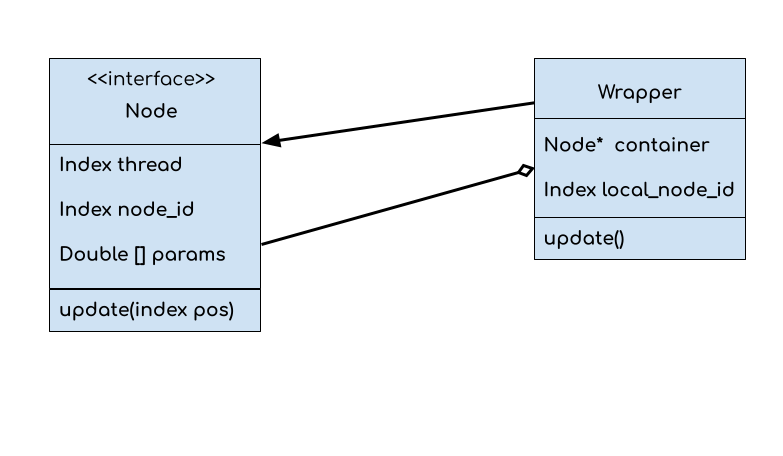
\includegraphics[width=0.8\textwidth]{src/pic/wrapper.png}
\caption{The naive solution for Vectorization: The \texttt{Node} class in the \emph{NestKenel} is adjusted by extending all its functions by a new parameter indicating the \texttt{local\_id} of the node that we want to apply the function on. Additionally, the attributes in the \texttt{Node} class are modified to have a vector from. The \texttt{Wrapper} class inherits from the \texttt{Node} class and at the same time has an attribute with a \texttt{Node} type. This makes the \texttt{Wrapper} class have an instance of itself, and we should definitely avoid using this design.}
\label{fig:naive}
\end{figure}

The \autoref{fig:naive} shows the relation between the \texttt{Node} and \texttt{Wrapper} classes. Here we have a cyclic dependency between the \texttt{Wrapper} and the \texttt{Node} class, as the \texttt{Wrapper} inherits from the node and at the same time it stores an instance of the \texttt{Node} class, which forces us to change the signature of the functions in  the \texttt{Node} class and makes the \texttt{Wrapper} have a twice the number of function as in the \texttt{Node} class. Those functions are with the extended \texttt{local\_id} parameter, and those without it. Definitely, this solution suffers from design problems, and it could make it hard for developer to maintain the logic and ensure a sound  and a correct implementation.

\section{The Container}

To solve the issue in the naive solution, we have to separate between \emph{vectorized} models and the already existing models. The context of which nodes must be retrieved and updated should be executed in blocks and in parallel without dependency between the nodes. Additionally, we have to avoid changing the declaration of the \texttt{Node} class functions to avoid the overhead of propagating these changes to the other derived classes from the \texttt{Node} class and make the implementation of the \emph{vectorized} models transparent to the \emph{NestKernel} components.



\begin{figure}[h!]
\centering
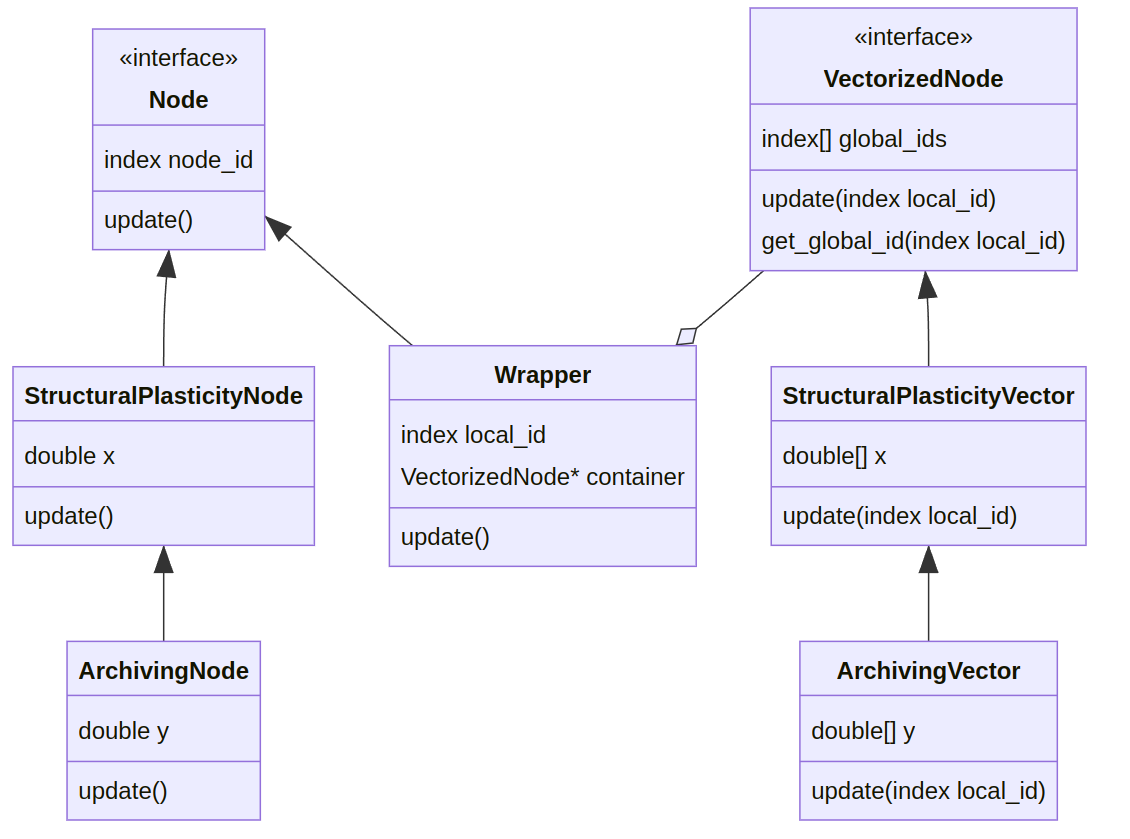
\includegraphics[width=0.8\textwidth]{src/pic/wrapper_node.png}
\caption{The Wrapper and the VectorizedNode: The new design after considering the drawbacks of the naive solution. The \texttt{Wrapper} still inherits from the \texttt{Node} interface, but instead of owning an attribute of the \texttt{Node} class, it owns an attribute of the \texttt{VectorizedNode}. The \texttt{VectorizedNode} class is the twin of the \texttt{Node} class, with the only difference that supports vectorization.}
\label{fig:container}
\end{figure}

In the \autoref{fig:container}, we illustrate the derived solution from the naive solution. The idea behind this solution is to split the \texttt{Wrapper} from the naive solution into two different classes. We have a new \texttt{Wrapper} class that inherits from the \texttt{Node} class, and it has a member variable of a \texttt{VectorizedNode} type. The \texttt{VectorizedNode}  is an interface that has the same exact functionality as the \texttt{Node} interface, with the only difference that all its member variables are vectors and all functions have an extra parameter which represents the position of the entry that we want to retrieve or update. Instead of having $n$ instances of the \texttt{Node} class from any arbitrary model, we have a single container instance from  the \texttt{VectorizedNode} that has vectors of size $n$ and each of these entries are represented by the \emph{Wrapper}. Since the \texttt{Wrapper} inherits from the \texttt{Node} class, the other component in the \emph{NestKernel} can then interact with the \texttt{Wrapper} without any further adjustments. Each call to the functions inside the \texttt{Wrapper} are forwarded to the \texttt{VectorizedNode} that exactly call the corresponding function with the \texttt{local\_id} as the context coming from the \texttt{Wrapper} instance. It is also important to notice that for each of the \texttt{StructuralPlasticitiyNode} and the \texttt{ArchivingNode} we have the equivalent vectorized class derived from the \texttt{VectorizedNode} that has the same functions but with the support for vectorized models.


\begin{figure}[h!]
\centering
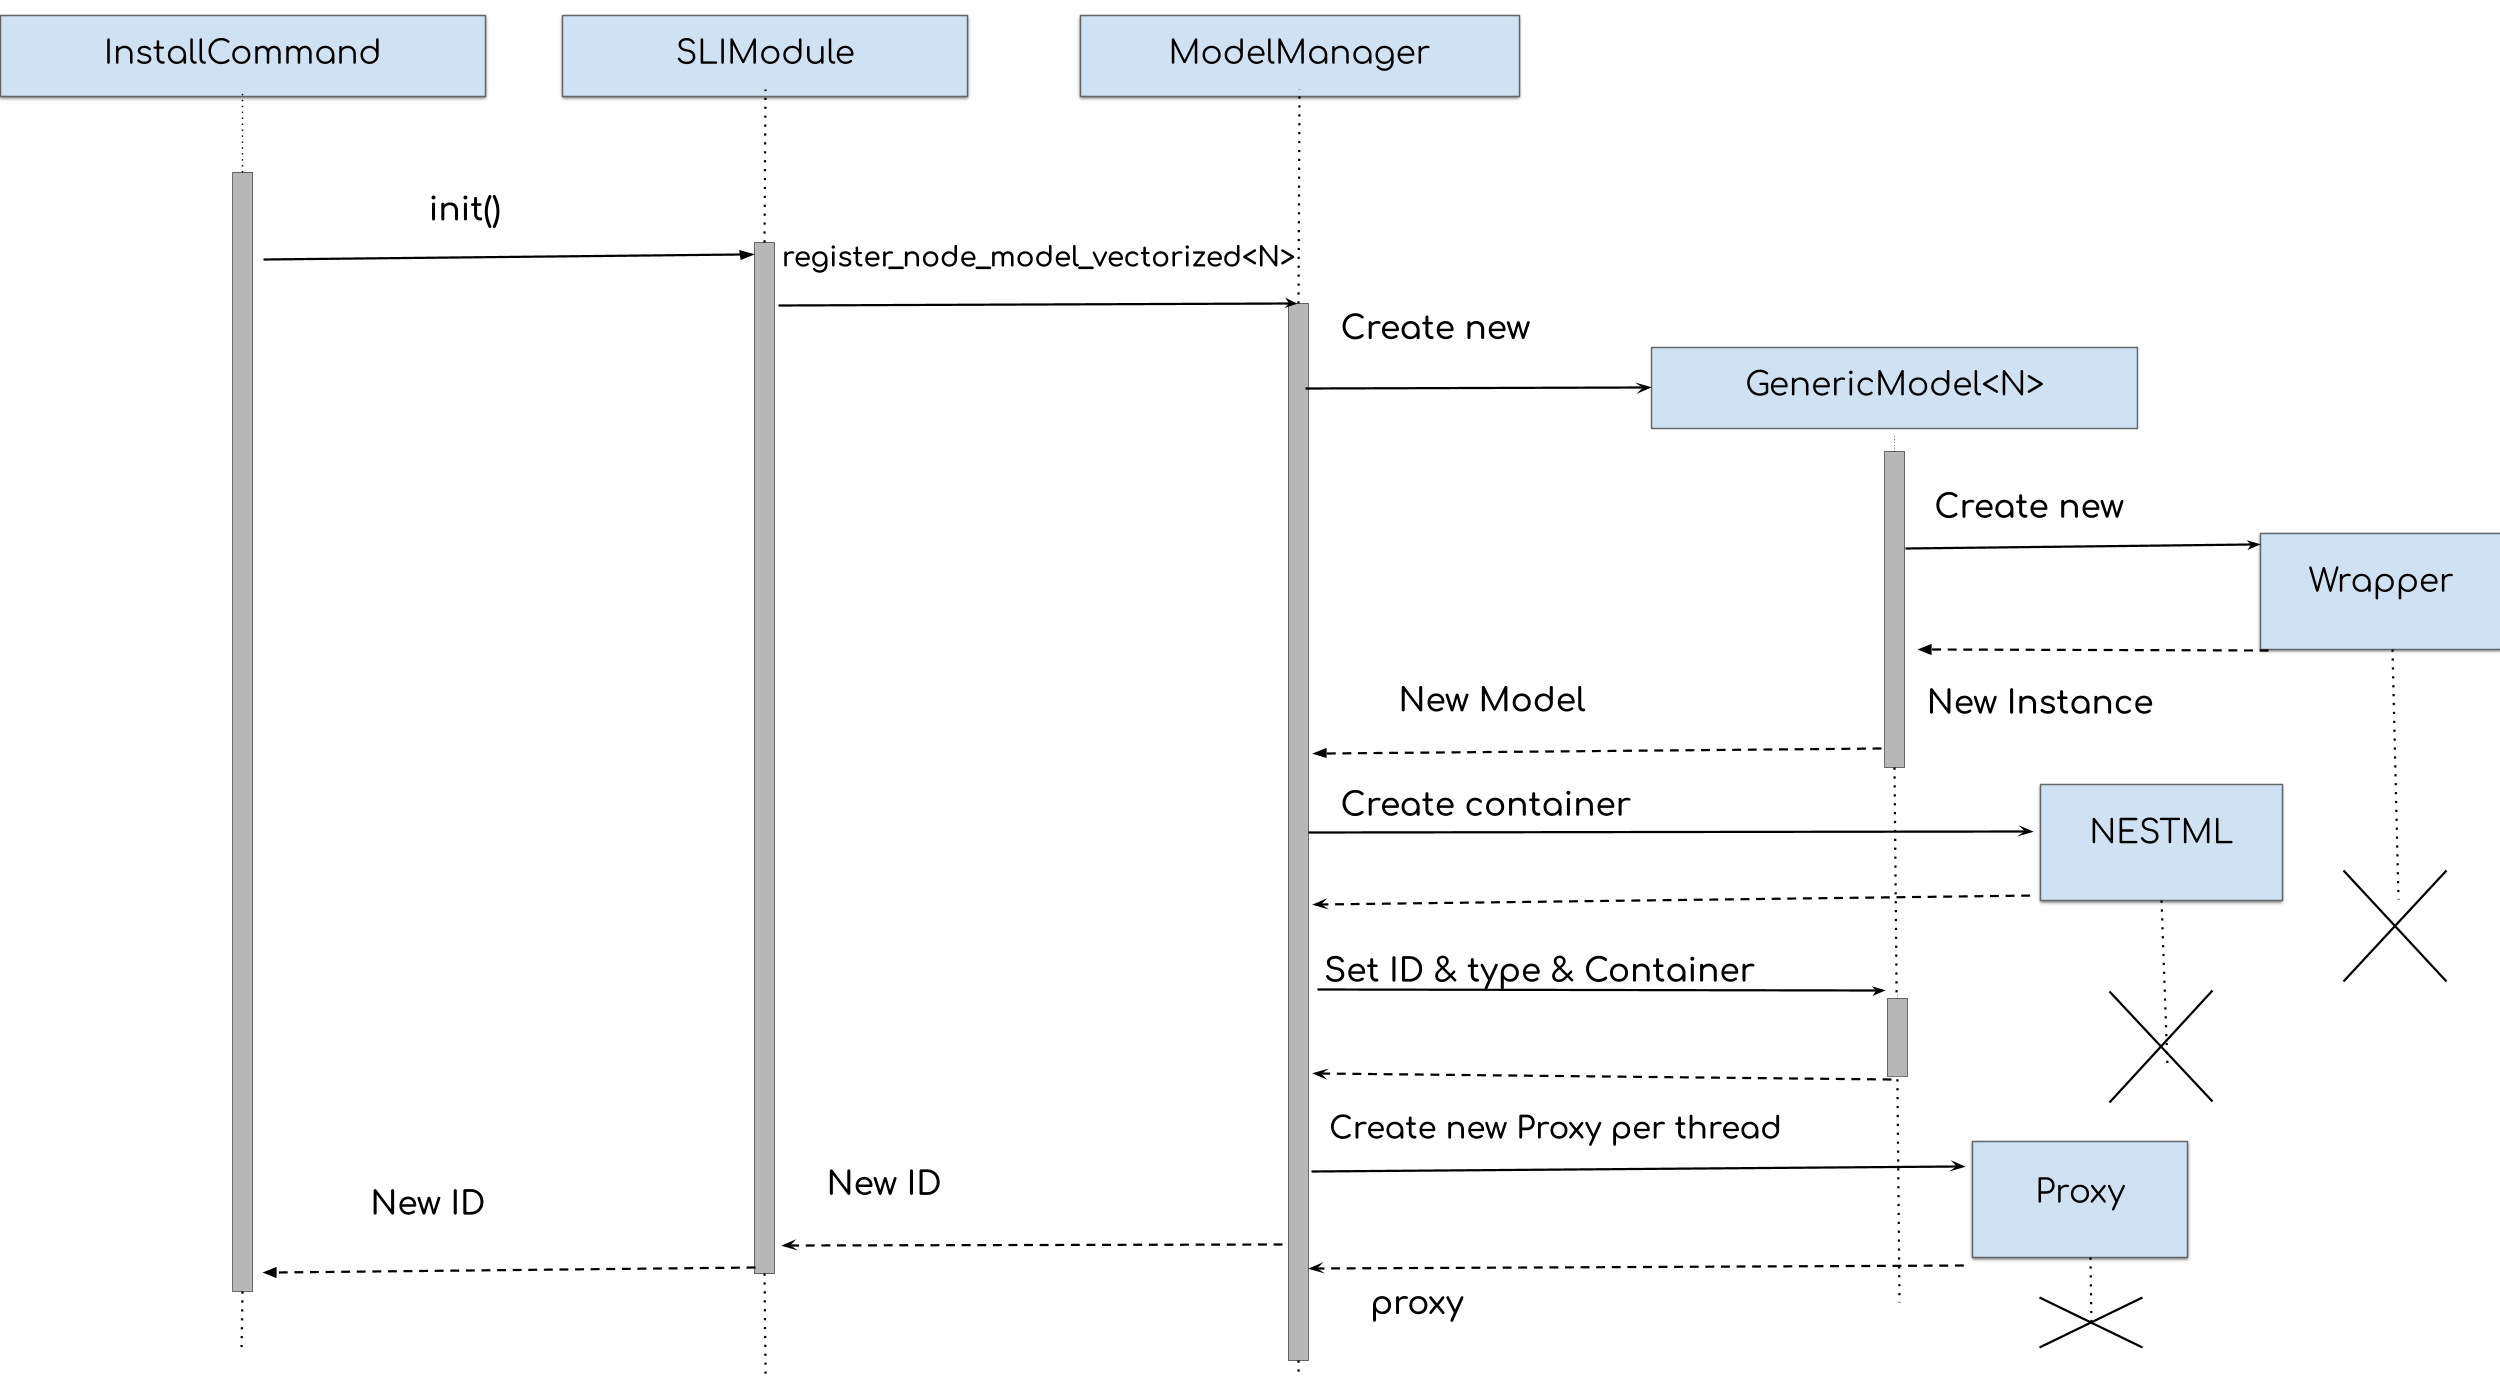
\includegraphics[width=\textwidth]{src/pic/node_creation_vec.png}
\caption{Registering a Vectorized model: The message sequence chart depicts the interaction between the components in the \emph{NestKernel} responsible for registering the vectorized new custom models.}
\label{fig:register_container}
\end{figure}

As depicted in the \autoref{fig:register_container}, registering new external models in the \emph{NestKernel} starts with calling the \texttt{register\_node\_model\_vectorized} function in the \texttt{ModelManager}. The function creates then a new instance of the \texttt{GenericModel}, but instead of providing the model class type as the value of the template \texttt{T}, we set \texttt{T} to the \texttt{Wrapper}. In other words, we create an instance from the \texttt{GenericModel<Wrapper>}. An instance of the \texttt{Wrapper} is created and stored locally in the \texttt{GernericModel}. Next, once the constructor of the \texttt{GernericModel} finishes, the control returns to the \texttt{register\_node\_model\_vectorized}, we proceed by creating an instance of the \texttt{VectorizedNode} which is indicated as \texttt{NESTML} in the figure. We create the container from the \texttt{VectorizedNode} and then update the created model by setting its \texttt{id}, \texttt{type} and \texttt{container}. Afterwards, as in the normal registration workflow, we just create the \texttt{Proxy} models for each thread which is not affected by the vectorization. In short, the main difference between registering a normal model and vectorized model is the in the provided class type \texttt{T} in \texttt{GenericModel} with the extra step of creating the container as an instance of the \texttt{VectorizedNode} class, otherwise everything stays the same.


In the typical way of running a simulation with external simple models without the \emph{vectorization} feature, there is am important condition that must be satisfied between the created nodes and the current number of used threads. The condition states that each node exactly belongs to one thread and threads can not modify the state of nodes coming from different threads. Since the \texttt{VectorizedNode} behaves the same as the \texttt{Node} class, then the same must hold for containers. Each container must belong exactly to one thread, and threads can only modify the containers they possess. In order for the \texttt{VectorizedNode} to fulfill this requirement, we have slightly modified the \texttt{Model} Class and the \texttt{ModelManager} in the \texttt{add\_neurons\_} function.\\


\begin{figure}[ht!]
    \centering
    \lstset{language=C++,
                keywordstyle=\color{blue},
                stringstyle=\color{red},
                commentstyle=\color{green},
                morecomment=[l][\color{magenta}]{\#}
}
\begin{lstlisting}[caption=Assigning containers to threads,frame=tlrb, label=lst:thread_container]{Name}
 if ( model.get_uses_vectors() )
      {
        if ( model.has_thread_assigned( t ) )
        {
          index t_container_pos = model.get_node_pos_in_thread( t );
          t_container = vectorized_nodes.at( t ).at( t_container_pos );
        }
        else
        {
          t_container = model.get_container()->clone();
          t_container->set_thread( t );
          vectorized_nodes.at( t ).push_back( t_container );
          index t_container_pos = vectorized_nodes.at( t ).size() - 1;
          model.add_thread_node_pair( t, t_container_pos );
        }
      }
      
\end{lstlisting}
\end{figure}

The \autoref{lst:thread_container} shows the inserted new functionality in the \texttt{add\_neurons\_} function for creating new \texttt{Node} instances from the registered models. We first start by checking if the model class supports \emph{vectorization}, and if it is the case, then we ask the model instance if it had seen the current running thread $t$ or not. If the model knows the thread $t$, then an instance of the \texttt{VectorizedNode} was already created. In that case, we simply ask the model to give us the position of the container in the thread $t$ and we retrieve it in order to resize it and adjust it accordingly. If the model has not seen the thread yet, then we simply \emph{clone} the container that is stored inside the model. Once the container is cloned, we update the container by providing  the thread $t$ that is owning it and also insert the container in the thread context. To simplify the matching between containers and threads, we simply have an attribute called \texttt{vectorized\_nodes} in the shape of \texttt{vector<vector<VectorizedNode>>}, so that the first dimension is occupied with the \texttt{thread\_id} and the second dimension with the created containers. The created container $c$ within the thread $t$ is then stored as \texttt{vectorized\_nodes.at(t).push(c)}, and the thread is registered in the container by simply calling \texttt{container.set\_thread(t)}. Once the matching between the container and the thread is completed, we then register the thread $t$ in the model instance, so that by the next call, the model knows which container to retrieve and at which position.  For models that do not support \emph{vectorization}, the whole new inserted block is ignored and the function \texttt{add\_neurons\_}  continues to execute without further changes. Since the \texttt{Wrapper} inherits from the \texttt{Node} class, the \texttt{create} function inside the model always returns an instance from the provided class \texttt{T} inside the \texttt{GenericModel<T>} class, which can be either the registered model without \emph{vectorization} or the new \texttt{Wrapper} class. As depicted in \autoref{lst:creating_nodes_while}, we almost change nothing in the \texttt{while-loop}, and instead of updating the container step by step, we simply wait until the while loop finishes and then update the container at once to save us the overhead of repeatedly calling the \texttt{resize} function.\\


\begin{figure}
    \lstset{language=C++,
                keywordstyle=\color{blue},
                stringstyle=\color{red},
                commentstyle=\color{green},
                morecomment=[l][\color{magenta}]{\#}
            }
\begin{lstlisting}[caption=Creating nodes,frame=tlrb, label=lst:creating_nodes_while]{Name}
 while ( node_id <= max_node_id )
      {
        Node* node = model.create( t );

        node->set_container( t_container );
        node->set_node_id_( node_id );
        node->set_nc_( nc_ptr );
        node->set_model_id( model.get_model_id() );
        node->set_thread( t );
        node->set_vp( vp );
        node->set_initialized();

        local_nodes_[ t ].add_local_node( *node );

        node_id += num_vps;
        has_at_leat_one_node = true;
      }

      local_nodes_[ t ].set_max_node_id( max_node_id );
      if ( t_container and has_at_leat_one_node )
      {
        t_container->resize( max_new_per_thread, t );
      }
    }
\end{lstlisting}
\end{figure}

\section{Limitation}

So far, we only made \emph{Vectorization} work with \emph{multithreading}, and we are still required to completely integrate it into the \emph{NestKernel}. We have implemented the \texttt{VectorizedNode} class that represents a container holding  \emph{vectors}, and the size of these vectors is the number of created \texttt{Wrapper} instances pointing to the container. For simplicity, we can consider the container as an \emph{array} and the \texttt{Wrapper} instances represent each entry in the array. Thus, each \texttt{Wrapper} can only modify the entry is pointing to. Right now, when we are updating the \texttt{Node} instances, we are iterating over each one of them individually. For the normal models without vectorization, we can not do anything about it, but for the vectorized models, we should aggregate the \texttt{Node} (i.e., \texttt{Wrapper}) instances that share the same container and then only apply the function we want on the container. Assume we have $n$ containers and each container has $k$ \texttt{Wrapper}s pointing to it, and we have a function $f$ that is applied to these items separately. In total, the function will be called $n\cdot k$ times, and for a large $k$ that might be a huge overhead. Instead, we can aggregate the items and only call the function $f$ $n$ times. Thus, each container can fully utilize the \emph{vectorization} by applying internally the function $f$ in parallel to the $k$ items.


Also, the \texttt{get\_status} and \texttt{set\_status} functions do not fully utilize the implemented new data structure for \emph{Vectorization}. Assume the container has $n$ vectors of size $k$ ($k$ is the number of attributes in the model). The normal execution of these functions takes each \texttt{Node} instance individually and iterates over the $k$ attributes and returns a \emph{dictionary} containing the values of the $k$ attributes. This workflow does not work well with \emph{vectorization}, because if  each \texttt{Wrapper} within the same container executes the same logic, then we might have a high number of \emph{cache misses}. Assume we have two consecutive access $x_i$ and $x_{i+1}$, and we have $k$ large enough so that not all vectors can be loaded into the registers. The \texttt{Wrapper} at position $x_i$ loads its necessary data and returns the \emph{dictionary}, the second \texttt{Wrapper} $x_{i+1}$ on the other hand must load the first $k$ vectors again. What really should happen is that each of the $l$ vectors must be loaded once in the registers. Since we have a consecutive access, all the entries must be loaded and ready to be used for constructing the result. Better yet, we simply again group the \texttt{Wrapper} instances by  the container type and let the container call these functions and treat each of these $k$ vectors individually and in parallel.

\cleardoublepage
